\section{Deep Learning Concepts}
\label{sec:deep-concepts}

\subsection*{Natural Language Processing}
\label{sssec:nlp}

Natural Language Processing (NLP) is a field of artificial intelligence that develops algorithms to enable machines to process, interpret, and generate human-like text. NLP empowers computers to perform language-related tasks traditionally requiring human intelligence, including Language translation, Sentiment analysis, Text classification, Information extraction


A key advancement in NLP has been the development of \textit{word embeddings} - numerical representations that capture semantic meaning and contextual relationships between words. These embeddings form the foundation for modern language understanding systems.



\subsection*{Word Embeddings}
\label{sssec:word-embeddings}

Word embeddings are vector representations of words. The challenge they aim to address is the ability to represent similar words—i.e., words that often appear in similar contexts—with similar vectors, where the vector directions also carry semantic meaning. 

While word vectors had been previously used in information retrieval, one of their most pivotal applications was their integration into neural networks. The need for word embeddings became evident when researchers began feeding words into Neural Networks (NNs).

Several encoding strategies were considered:

\begin{itemize}
    \item \textbf{Character-based representation:} Training a character-level model consumes a large portion of the network's capacity to simply learn valid word forms, potentially limiting its ability to learn higher-level features such as context or semantics.
    
    \item \textbf{Dictionary-based representation:}
    \begin{itemize}
        \item \textit{One-hot encoding:} Each word is represented as a vector of length $N$ (the vocabulary size) with all entries set to 0 except for a 1 in the position corresponding to that word. This approach does not encode similarity and leads to sparse and high-dimensional data, which is inefficient.
        
        \item \textit{Index-based encoding:} Assigning a unique integer to each word implies false assumptions—e.g., that adjacent indices mean semantic closeness.
    \end{itemize}
\end{itemize}

These limitations highlighted the need for richer numerical representations that reflect both word meaning and context. Additionally, words can have multiple meanings in different contexts, motivating dynamic or multi-context embeddings.

\subsubsection*{Popular Embedding Models}

\begin{itemize}
    \item \textbf{Word2Vec:} This model learns embeddings by predicting context words given a target word (Skip-Gram) or predicting a word from its context (Continuous Bag-of-Words, or CBOW). Word2Vec optimizes training speed and scalability through techniques like \textit{Negative Sampling}. It excels at capturing local context and performs well on tasks like word prediction.
    
    \item \textbf{GloVe (Global Vectors):} GloVe is an unsupervised learning algorithm that constructs a co-occurrence matrix capturing the frequency with which word pairs appear together in a corpus. It then factorizes this matrix to produce dense word vectors. GloVe captures both local and global context but may struggle with tasks involving polysemous words (words with multiple meanings).
\end{itemize}

\subsubsection*{Vector Analogies}

Word embeddings allow for interesting arithmetic operations that reveal semantic relationships. A well-known example illustrates this with gender analogies:

\begin{quote}
\centering
\texttt{vector("king") - vector("man") + vector("woman") $\approx$ vector("queen")}
\end{quote}

This vector analogy demonstrates that the learned embedding space encodes meaningful relationships such as gender differences, enabling analogical reasoning.

\begin{figure}[htbp]
  \centering
  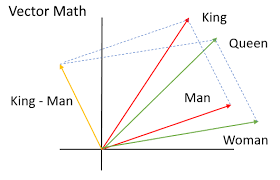
\includegraphics[width=0.5\textwidth]{images/Word Embedding Example.png}
  \caption*{\textbf{Figure 1:} The classical \textit{king - man + woman = queen} example of word embeddings.} % Starred version
  \label{fig:indexing-process-manual}
\end{figure}

Word embeddings are widely used in NLP tasks such as sentiment analysis, machine translation, and question answering. Interestingly, research has shown that source code exhibits similar co-occurrence patterns to natural language. As a result, vector representations of tokens in programming languages have also been explored using similar embedding techniques.

\subsection*{Audio Embeddings}
\label{sssec:audio-embeddings}

Audio embeddings are numerical representations of audio samples that capture essential characteristics and features of the sound. These embeddings are widely used in applications such as audio classification, music recommendation, and speech recognition. Essentially, an audio embedding transforms complex audio data into a fixed-size vector, making it easier for machine learning models to analyze and compare different audio samples. This compact vector encodes information such as pitch, rhythm, timbre, and other auditory features.

The process of generating audio embeddings typically involves several steps:

\begin{itemize}
    \item \textbf{Pre-processing:} The raw audio signal is first pre-processed. Common steps include noise reduction, normalization, and segmentation into smaller chunks or frames.
    
    \item \textbf{Feature extraction:} From the pre-processed audio, features are extracted using techniques such as:
    \begin{itemize}
        \item \textit{Short-Time Fourier Transform (STFT)}
        \item \textit{Mel-Frequency Cepstral Coefficients (MFCC)}
        \item \textit{Mel-spectrograms}
    \end{itemize}
    These methods help capture the frequency content of the audio over time, allowing models to encode meaningful auditory information.
    
    \item \textbf{Embedding generation:} Machine learning models such as Convolutional Neural Networks (CNNs) or Recurrent Neural Networks (RNNs) are applied to the extracted features to produce dense vector embeddings. 
\end{itemize}

For instance, CNNs may learn to recognize different instruments or environmental sounds, while RNNs can capture temporal patterns in speech or music. The resulting embedding is a fixed-size vector that summarizes the most relevant properties of the audio sample.

These audio embeddings are then used for downstream tasks such as clustering, retrieval, or classification, enabling systems to interpret and manipulate audio data effectively in various contexts.

\subsection*{Large Language Models}
\label{sssec:llms}

A language model is a statistical representation of a human language, capable of estimating the likelihood of word sequences based on the text data it was trained on.

In their most advanced form, \textit{Large Language Models} (LLMs) are a fusion of feedforward neural networks and transformers. LLMs are characterized by three major features:

\begin{itemize}
    \item \textbf{Scale:} LLMs are trained on extremely large datasets and have a vast number of parameters, often exceeding one billion.
    \item \textbf{General-purpose capabilities:} These models are capable of performing a wide range of tasks, including language generation, summarization, translation, question answering, and even solving mathematical problems.
    \item \textbf{Fine-tuning potential:} Although LLMs are trained on general data, they can be fine-tuned for specific tasks using much smaller, task-specific datasets.
\end{itemize}

LLMs leverage Deep Learning (DL) techniques—particularly the transformer architecture—to capture the complex dependencies and hierarchical structures present in natural language. Notable examples include \textit{GPT-3} (Generative Pre-trained Transformer 4) and \textit{Llama 3.2}.

The emergence of transformers has played a critical role in the development of LLMs, enabling them to understand and generate human-like text with high fluency and contextual awareness. Transformers are now the standard architecture underlying most modern LLMs.

\subsection*{Transformers}
\label{sssec:transformers}

Transformers are a Neural Network architecture that have revolutionized Natural Language Processing (NLP). Neural Networks are capable of analyzing vast amounts of data, including images, videos, text, and audio. Each data type is best suited for specific neural architectures; for instance, Convolutional Neural Networks (CNNs) are optimized for visual data.

CNNs simulate how the human brain processes visual information and are particularly powerful for tasks like object detection, facial recognition, and handwritten text recognition. However, for language-related tasks, CNNs were not the most effective.

To address this, Recurrent Neural Networks (RNNs) were developed for handling sequential data, as shown in Figure~\ref{fig:rnn_architecture}. RNNs could capture temporal dependencies and were widely used for language modeling tasks. However, they struggled with long-term dependencies due to issues like the vanishing and exploding gradient problems. This made them difficult to train and limited their ability to remember information across long sequences.

\begin{figure}[htbp]
  \centering
  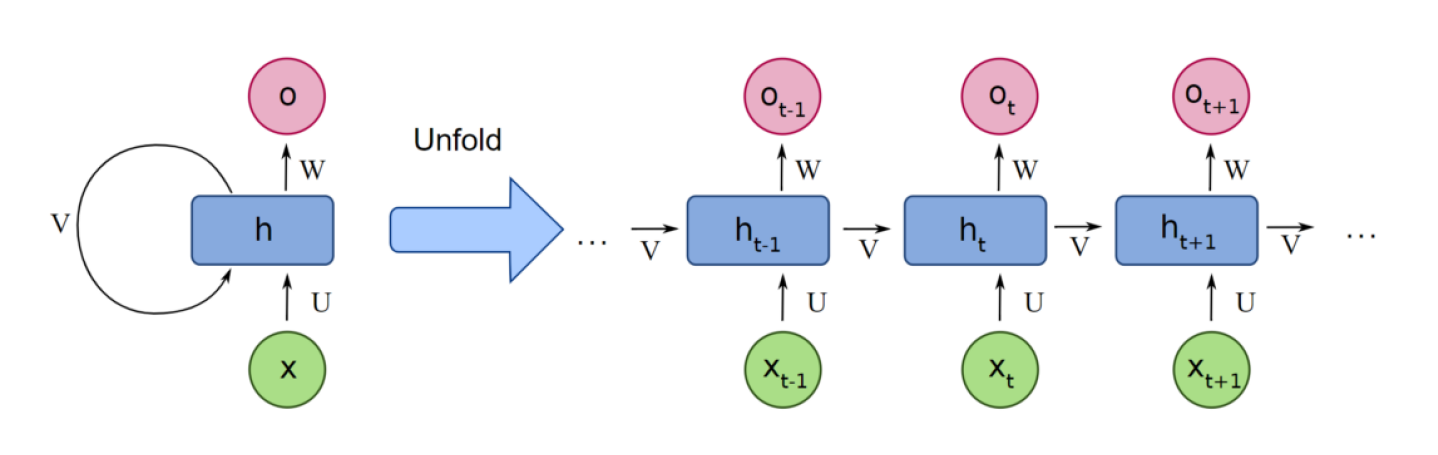
\includegraphics[width=1\textwidth]{images/RNN.png}
  \caption*{\textbf{Figure 1:} RNN Architecture} % Starred version
  \label{fig:rnn_architecture}
\end{figure}

In 2017, the introduction of Transformers by researchers from Google and the University of Toronto marked a significant breakthrough. Initially designed for translation tasks, the Transformer architecture has since become the standard for modern NLP models.

Unlike RNNs, Transformers can be easily parallelized, which allows for the training of extremely large models. The architecture of the Transformer is illustrated in Figure 2.

\begin{figure}[H]
  \centering
  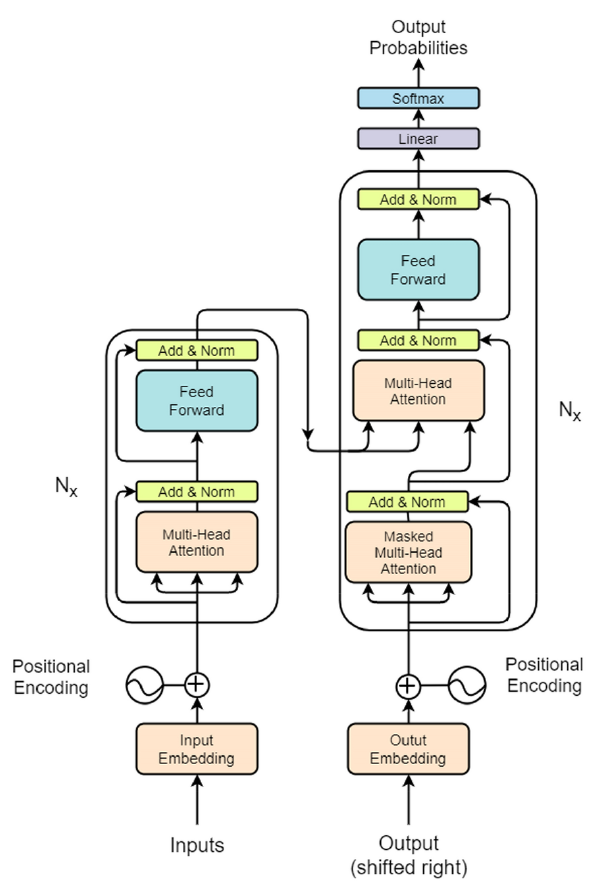
\includegraphics[width=0.55\textwidth]{images/Transformer Architecture.png}
  \caption*{\textbf{Figure 2:} Transformer Diagram from the original paper ``Attention is All You Need''} % Starred version
  \label{fig:transformer_architecture}
\end{figure}

Transformers are based on three key concepts:

\begin{itemize}
    \item \textbf{Positional Encodings:} Since Transformers do not process input sequences in order like RNNs, positional encodings are added to each word to preserve the sequence information. Originally, sinusoidal functions were used to generate these encodings, and the model learns to interpret them during training.

    \item \textbf{Attention:} Introduced in 2015, the attention mechanism assigns a contextual weight to each word in the input, allowing the model to focus on the most relevant parts of a sentence. This is not based solely on individual words, but on the entire context.

    \item \textbf{Self-Attention:} This is a special form of attention where the model considers the same input sequence to compute the relationships between its elements. Self-attention helps capture dependencies across the whole sequence simultaneously, ensuring that important information is retained throughout the process.
\end{itemize}

Not all Transformer models are the same. There are many architectural variations designed for specific tasks, such as BERT for masked language modeling, GPT for autoregressive generation, and T5 for text-to-text tasks. Despite these differences, they all share the same foundational principles of attention and positional encoding.

\subsection*{Retrieval-Augmented Generation (RAG)}

Retrieval-Augmented Generation (RAG) is a hybrid architecture that combines the strengths of retrieval-based and generative models. Instead of relying solely on pre-trained knowledge, RAG enhances a generative language model by incorporating external documents retrieved from a large corpus in real time.

The architecture consists of two main components:

\begin{itemize}
    \item \textbf{Retriever:} Fetches relevant documents or passages based on the input query, typically using dense or sparse retrieval methods.
    \item \textbf{Generator:} A language model that conditions its output on both the input query and the retrieved documents to generate accurate and informative responses.
\end{itemize}

RAG is particularly useful in knowledge-intensive tasks such as question answering and summarization, where grounding the output in factual information is crucial.


\subsection*{CLAP (Contrastive Language-Audio Pretraining)}

CLAP is a neural network model designed to learn joint representations of audio and natural language. By employing contrastive learning techniques, CLAP aligns audio signals with their corresponding textual descriptions in a shared embedding space. This approach enables the model to perform tasks such as zero-shot audio classification, retrieval, and captioning without the need for task-specific training.

The architecture of CLAP consists of two main components:

\begin{itemize}
    \item \textbf{Audio Encoder:} Processes audio inputs, typically using a SWIN Transformer, to extract meaningful features from log-Mel spectrograms.
    \item \textbf{Text Encoder:} Utilizes models like RoBERTa to convert textual descriptions into feature representations.
\end{itemize}

Both audio and text features are projected into a common latent space, allowing the model to measure similarity between audio clips and textual inputs effectively. This design facilitates various applications, including audio-text retrieval and zero-shot classification, by leveraging the semantic alignment between modalities.
